\chapter{Konwolucyjne sieci neuronowe}
\textit{Konwolucyjne sieci neuronowe} (ang. \textit{Convolutional Neural Networks}) są biologicznie inspirowanymi sztucznymi sieciami neuronowymi. Podłoże pochodzi od badań nad korą wzrokową zapoczątkowanych w pracach Hubel'a i Wiesel’a w roku 1968 dotyczących widzenia kotów. Dzięki paracom neurofizjologów nauka o sztucznych sieciach rozwiajana od lat 40-tych XX wieku obrała obecny kierunek. Wiadomo, że kora wzrokowa zawiera złożone układy komórek. Komórki te odpowiadają za przetwarzanie informacji z regionów pola widzenia, tak żeby sumarycznie pokryć je w całości. Komórki te działają jak lokalne filtry przestrzeni wejściowej zaprojektowane, tak aby wydobyć istotne cechy z naturalnych obrazów. Dla przykładu reagują na orientację linii, kształty i kolory.

W zapisie cyfrowym wykorzystywanym najczęściej w przetwarzaniu obrazów metodami sztucznej inteligencji informację wejściową stanowi dyskretna \textit{funkcja obrazowa} $I$, która przypisuje kolejnym punktom obrazu tzw. \textit{pikselom} kolor zdefiniowany w zadanej przestrzeni barw np. RGB, CMYK, GrayScale (zob. [barwy]). W praktyce przetwarzania obrazów medycznych najczęściej spotyka się z dwuwymiarowe funkcje $I$($x$, $y$) lub trójwymiarowe $I$($x$, $y$, $z$).

Filtracje obrazów cyfrowych mające na celu wydobycie istotnych cech uzyskuje się za pomocą operacji splotu maski $K$ filtru z kolejnymi fragmentami obrazu I, co można zapisać następująco:
\begin{equation}
	I'\left(x, y\right) = \sum_{n=0}^{N} \sum_{k=0}^{N} I\left(x + n, y + k \right)K\left(n, k\right).
\end{equation}
Najczęściej spotykane wymiary masek $K$ to 3$\times$3 -- 11$\times$11. 

/*definicje krawędzi, kształtów, obiektów*/

Ewolucja sieci konwolucyjnych do obecnej postaci przebiegała stopniowo, a najważniejsze jej elementy zostały przedstawione w kolejnej sekcji. 

\section{Zarys historyczny}

Historia głębokich sieci neuronowe zaczęła się w latach 40-tych XX wieku. Pierwszy formalny model neuronu był zaproponowany przez Warrena McCulloch i Waltera Pitts w roku 1943 [Pitts]. Była to bramka logiczna, której wyjście stawało się aktywne w momencie, gdy liczba aktywnych wejść przekroczyła pewien zdefiniowany próg. 

Pierwsza architektura sieci neuronowej zawierająca wiele neuronów z ważonymi połączeniami między sobą została zaproponowana w 1957 roku przez Franka Rosenblatta [Perc]. Sieć, pokazaną na Rys. \ref{Perceptron} nazwano perceptronem, co związane było z zamiłowaniem jego twórcy do aplikacji związanych z percepcją, zwłaszcza mowy czy pisma. 
\begin{figure}[h!]
	\centering
	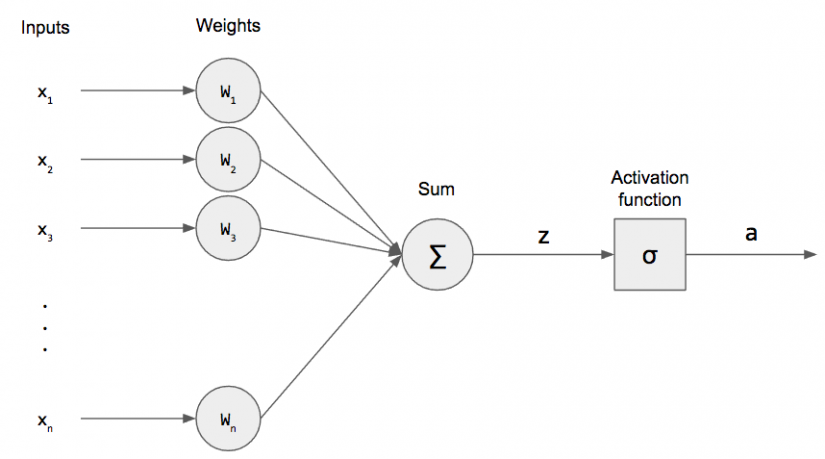
\includegraphics[width=0.55\textwidth]{figures/perceptron.png}
	\caption{Topologia perceptronu.}
	\label{Perceptron}
\end{figure}

Model neuronu zaproponowany przez Rosenblatta charakteryzuje się strukturą o wielu wejściach i jednym wyjściu. Sygnał wyjściowy $y$ ściśle zależy od sygnałów wejściowych $x_1$...$x_n$, a zależność ta, podana wzorem \ref{eqActFunc}, nazywana jest \textit{funkcją aktywacji neuronu}. 
\begin{equation}
\label{eqActFunc}
y=f\left(x_1, x_2,..., x_n\right)
\end{equation}
Funkcja $y$ ma za zadanie modelować biologiczne własności neuronu związane z warunkową propagacją sygnału nerwowego. Dla przykładu liniowa funkcja aktywacji neuronu realizowana jest sumą:

\begin{equation}
\label{eqLinActFunc}
y=\sum_{i=1}^{n}w_i x_i
\end{equation}

gdzie $w_i$ są to wagi wektora $w$ = ($w_1$,...,$w_n$). Wprowadzenia do perceptronu wag $w$ dało możliwość uczenia się architektury poprzez modyfikację ich wartości. Badania nad różnymi funkcjami aktywacji doprowadziły do wielu sukcesów modelu Rosenblatta. Wyszczególnić można zwłaszcza funkcję typu Sgmoid i ReLU.

/*Master algorithm użyj opisy S-curve tutaj w odniesieniu do rozwiązania problemu Minsky*/

Po blisko dekadzie badań nowej architektury w 1969 roku Marvin Minsky i Seymour Papert w książce \textit{Perceptrons} opublikowali listę problemów, których nie można było rozwiązać z użyciem perceptronu. Do najsławniejszych należał problem związany z brakiem możliwości modelowania funkcji XOR.

Dopiero w 1986 roku część z zarysowanych przez Minsky'ego i Paperta problemów udało się rozwiązać za sprawą pracy Davida Rumelharta, Geoffa Hintona i Ronalda Williams traktującej o praktycznym zastosowaniu opisanego w latach 70-tych algorytmu wstecznej propagacji, umożliwajacym trening perceptronów wielowarstwowych [Backprop]. Schemat takiej sieci zaprezentowano na Rys. \ref{MLperceptron}
\begin{figure}[h!]
	\centering
	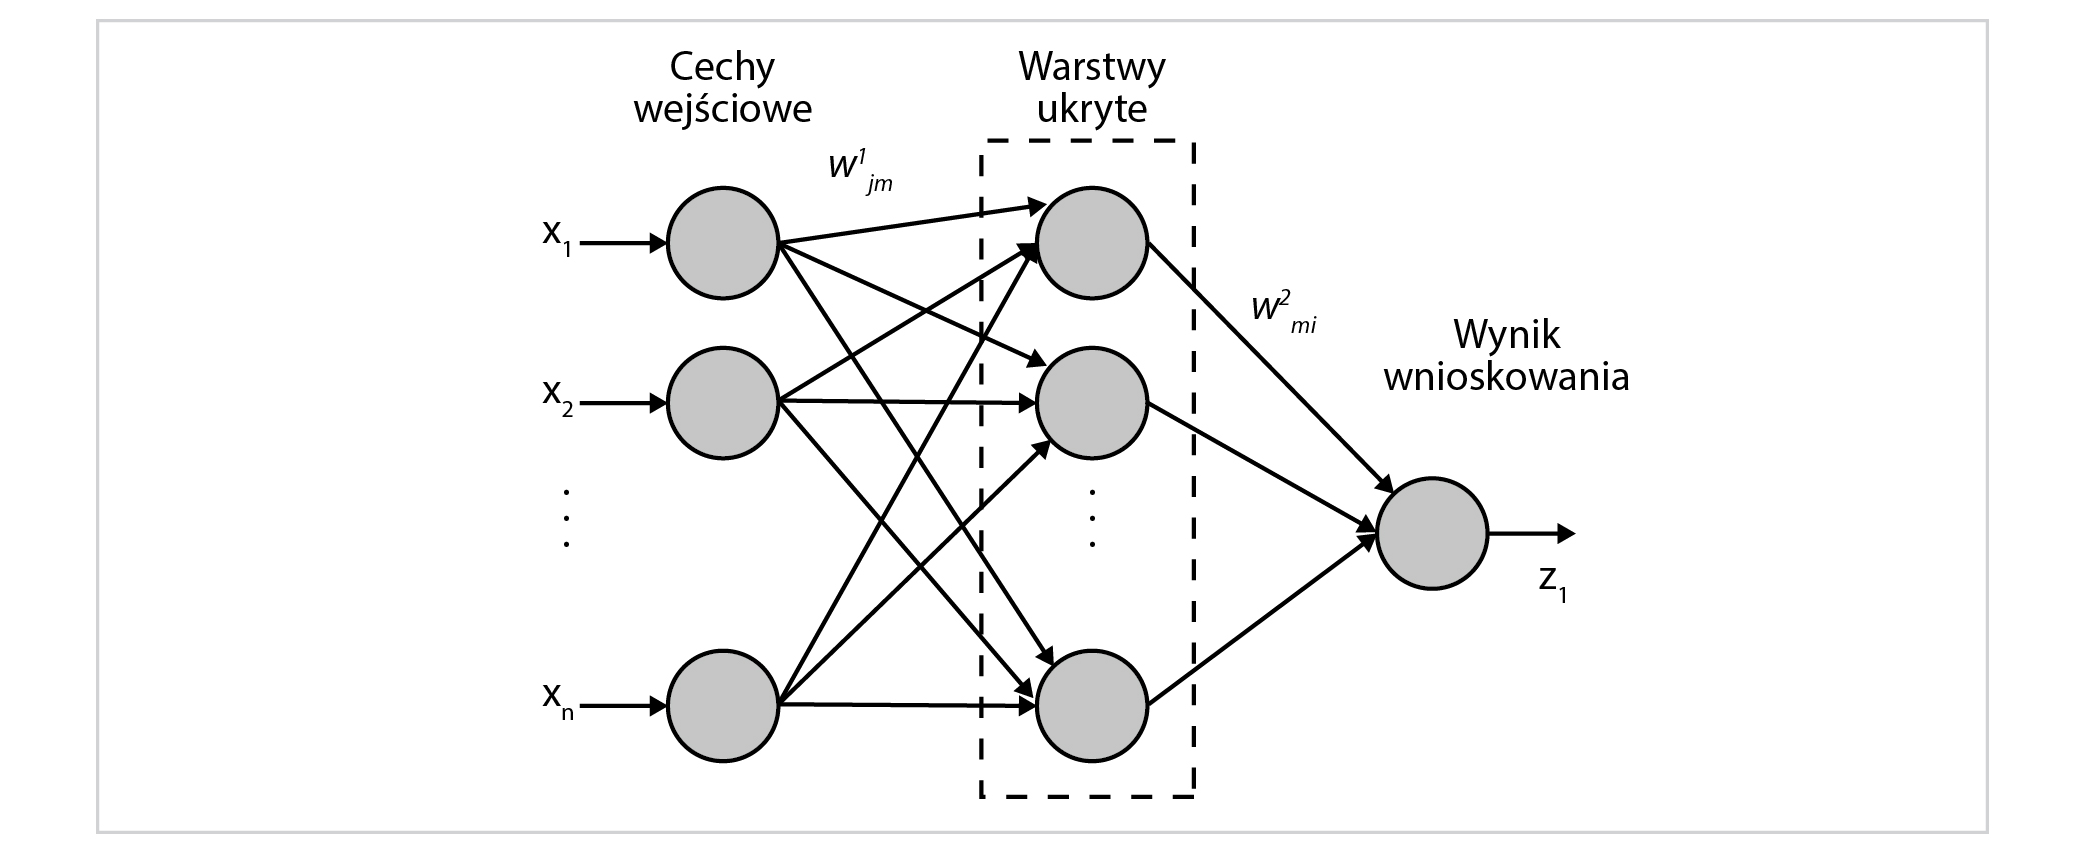
\includegraphics[width=0.55\textwidth]{figures/MLperceptron.png}
	\caption{Topologia perceptronu wielowarstwowego.}
	\label{MLperceptron}
\end{figure}

Z wykorzystaniem sieci wielowarstwowych możliwe stało się modelowanie funkcji XOR jak i innych problemów nieliniowych o praktycznym wymiarze. 

W 1989 roku, Yann LeCunn, były uczeń Geaoffa Hintona zaprezentował swoje badania z użyciem sieci wielowarstwowych do klasyfikacji odręcznego pisma [LeCun et al., 1989a]. Finalnie, badania te doprowadziły do przedstawienia w 1998 roku pierwszej sieci konwolucyjnej nazwanej LeNet [LeNet]. Architekturę tej sieci przedstawiono na Rys. \ref{LeNet}.
\begin{figure}[h!]
	\centering
	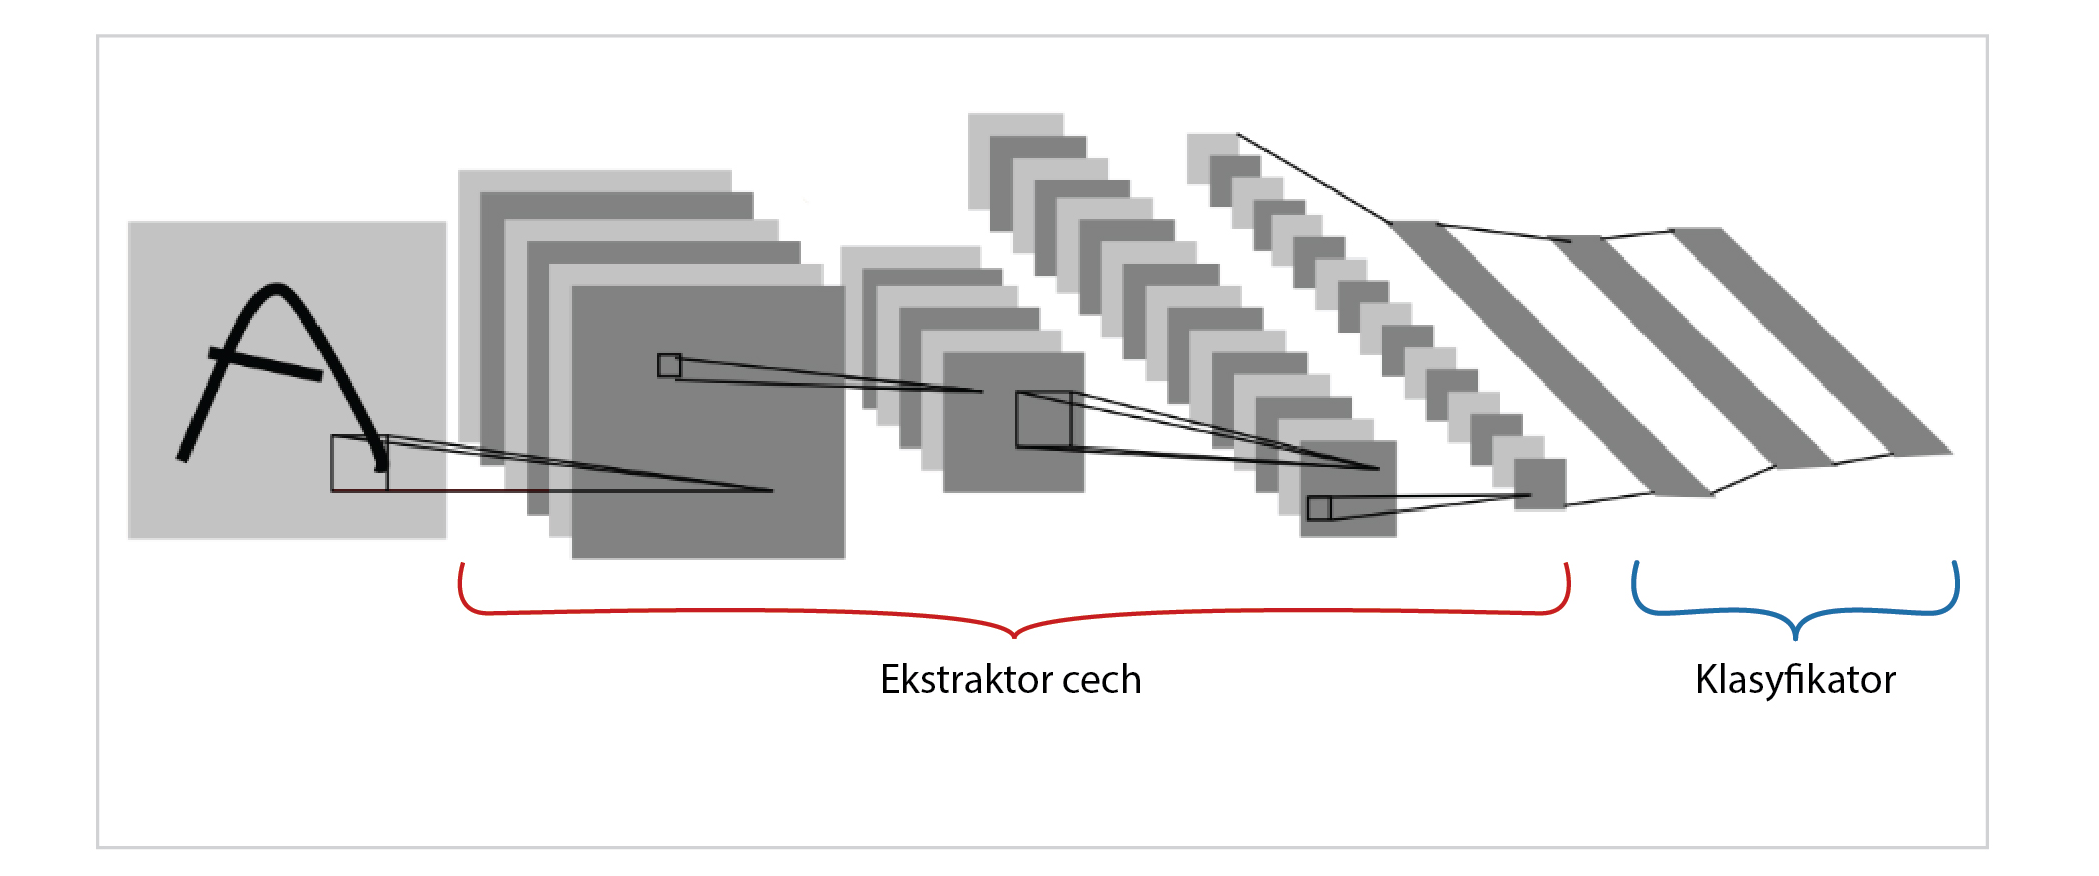
\includegraphics[width=1\textwidth]{figures/lenet.png}
	\caption{Topologia sieci LeNet.}
	\label{LeNet}
\end{figure}

Sieć składała się z 7 warstw i zawierała około 60,000 parametrów. Oryginalnie, sygnałem wejściowym sieci stanowił obrazek o wymiarach 32$\times$32.

W architekturze LeNet uwidoczniły się dwie podstawowe składowe współczesnych sieci konwolucyjnych tj. \textit{ekstraktor cech} -- zawierający filtry, których wartości parametrów masek są optymalizowane pod kątem wyboru cech charakterystycznych dla zadanego zbioru danych oraz \textit{klasyfikator} -- zawierający neurony z wagami, których wartości są optymalizowane w celu końcowego rozróznienia zbioru danych na podstawie wyekstrachowanego wczęsniej wektora cech. 

W uproszczeniu można opisać sieć konwolucyjną jako klasyczną topologię perceptronu wielowarstwowego poprzedzoną ciągiem bloków służących do automatycznej ekstrakcji cech obrazowych. Najczęściej bloki te składają się z \textit{warstw konwolucyjnych}, w których pogrupowane są filtry używane do ekstrakcji cech obrazowych różnego poziomu (np. krawędzie, kształty, obiekty), z opisanych wcześniej warstw aktywacji oraz warstwy typu \textit{pooling} realizujące nieliniową redukcję wymiarowości (np. max-pool wybiera największą wartość z danego obszaru obrazu\footnote{operacja max-pool jest najczęściej stosowaną operacją do nieliniowej redukcji wymiarowości, o innych można przeczytać w [poolingOps]}). Warstwy wykorzystane do klasyfikatora są \textit{warstwami w pełni połączonymi} (ang. \textit{fully connected}, w skr. \textit{FC}), a więc neuron z danej warswy jest połączony z każdym neuronem z warstwy następnej (LeNet miała 2 warstwy FC).

Pojedynczy splot filtru z obrazem wejściowym nazywany jest \textit{cechą} [OTR-19]. Cechy są bardzo łatwe do wizualizacji dlatego sieci konwolucyjne mogą być łatwiejsze do interpretacji niż inne algorytmy sztucznej inteligencji. W ostatnich latach powstało wiele algorytmów do wizualizacji wyników działania sieci konwolucyjnych np. Saliency Maps [OTR - 20], GradCam [OTR - 21] albo metody bazujące na skierowanych acyklicznych grafach [OTR - 22]. Grupy cech z wybranego obszaru obrazu wejściowego, połączone w reprezentacje na róznych warstwach konwolucyjnych tworzą \textit{mapy cech}. Dla przykładu w LeNet każda z warstw zawierała po odpowiednio: 6, 6, 16, 16 i 120 map cech o różnych wymiarach. 

Złożoność budowy sieci konwolucyjnych oraz duża liczba parametrów spowodowała szereg wyzwań związanych z praktycznym ich wykorzystaniem m.in. poprawną klasyfikacją zbioru danych. Najważniejsze z wyzwań zostały opisane w kolejnej sekcji.  

\section{Szkolenie głębokich sieci neuronowych}

Wiekszość algorytmów szkolenia głębokich sieci neuronowych obejmuje zadanie \textit{optymalizacji}, rozumiane jako minimalizację, bądź maksymalizację \textit{funkcji celu} $f$($x$) przez zmianę $x$. W literaturze można też znaleźć inne nazwy funkcji celu takie jak \textit{kryterium}, \textit{funkcja kosztów}, \textit{funkcja strat}, \textit{funkcja błędów} (za [DL-IANGoodfellow]). 

Podczas zadania optymalizacji bardzo często wykorzystuje się \textit{pochodną funkcji} oznaczaną jako $f'$($x$) lub $\frac{\delta y}{\delta x}$, gdyż niesie ona informacje o nachyleniu funkcji w punkcie $x$. W praktyce funkcje celu są wielowymiarowe dlatego wykorzystywane są \textit{pochodne cząstkowe} informujące o nachyleniu w poszczególnych wymiarach. Wektor zawierający pochodne cząstkowe funkcji nazywany jest \textit{gradientem} i oznaczany jako $\bigtriangledown f$($x$). Dodatkowo czasami istnieje konieczność znalezienia wszystkich pochodnych cząstkowych funkcji, której wejście i wyjście stanowią wektory. Taka macież nosi nazwę \textit{macierzy Jacobiego}, natomiast macierz \textit{drugich pochodnych} cząstkowych (tj. pochodnych pochodnych) \textit{macierzą Hessego}.

Metody optymalizacji bazujące na wartości gradientu w kolejnych krokach iteracji obierają kolejne wartości funkcji $f$ przesuwając się w kierunku spadku gradientu:
\begin{equation}
x' = x - \epsilon \bigtriangledown f(x),
\end{equation} 
gdzie $\epsilon$ to \textit{szybkość uczenia się}, parametr określający wielkość kroku. 

Funkcja celu w przypadku praktycznych zadań optymalizacyjnych, wykorzystujących głębokie uczenie się jest zazwyczaj \textit{funkcją złożoną}, a zatem efekt jej działania jest równoważny operacją wykonywanym przez szereg funkcji. Do obliczeń pochodnych funkcji złożonych z funkcji, których pochodne są znane stosuje się tzw. \textit{regułę łańcuchową}. Przypuśćmy, że y = g(x) i z = f(g(x)) = f(y), $x$ i $y$ to wektory. Wówczas regułę łańcuchową można zapisać jako:
\begin{equation}
\frac{\delta z}{\delta x_i} = \sum_{j} {\delta z}/{\delta y_j}{\delta y_j}/{\delta x_i}, 
\end{equation}
co w zapisie wektorowym równoważne jest z równaniem:
\begin{equation}
\bigtriangledown_x z = \left({\delta y}/{\delta x}\right)^T \bigtriangledown_y z, 
\end{equation}
gdzie $\frac{\delta y}{\delta x}$ to macierz Jacobiego. Regułę tak zapisaną prosto uogólnie się do zmiennych tensorowych (zob. IanGoodf-205). 

Można zatem gradient zmiennej $x$ otrzymać przez pomnożenie macierzy Jacobiego przez gradient $\bigtriangledown_y z$. W tym celu w metodach głębokiego uczenia się wykorzystuje się algorytm \textit{propagacji wstecznej}, który oblicza regułę łańcuchową w wydajnej kolejności stosując działania w grafie (zob. [Backprop]).

 /*SGD, ADAM, */
-pakiety, liczenie gradientu na pakietach zapewnia wydjaność 
/*FP, TP, FN, TN*/
/*Normalizacja*/

Wraz z rozwojem metod sztucznej inteligencji, w tym konwolucyjnych sieci neuronowych pojawiały się problemy związane z poprawną klasyfikacją zbiorów danych. Dwa najważniejsze tj. problem nadmiernego dopasowania i redukcji wymiarowości zostaną przedstawione w kolejnych sekcjach.

\subsection{Problem nadmiernego dopasowania}
\label{sec-overffiting}

Jak wiadomo proces uczenia się sieci ma na celu najlepsze możliwe przybliżenie docelowej klasyfikacji bazując na danych przykładach, czyli zbiorze uczącym $U$. Dążenie do najlepszego możliwego przybliżenia zbioru $U$ wprowadza niepożądane zjawisko zwane \textit{nadmiernym dopasowaniem}. Wtedy to dokładność klasyfikacji zbioru $U$ jest wysoka lub nawet bezbłędna, natomiast znacznie niższa jest dokładność klasyfikacji zbioru testowego $T$ i walidacyjnego $W$ zawierającego przykłady inne niż w $U$. W praktyce oznacza to, że model staje się mało użyteczny, gdyż nowe dane nie są poprawnie klasyfikowane.

Z uwagi na ten fakt ogólnym dążeniem w procesie uczenia się sieci jest osiągnięcie \textit{maksymalnej generalizacji} klasyfikacji. Sieć o wysokim współczynniku generalizacji lepiej klasyfikuje ogół zadanych wekto-
rów wejściowych niż sieć, która ma niski współczynnik generalizacji i jest nadmiernie dopasowana do zbioru $U$.

W celu uzyskania generalizacji należy wybrać taki model klasyfikatora, który wystarczy do zachowania
poprawnej klasyfikacji w mocy. Empirycznie ustalane są zatem maksymalnie ogólne, dostateczne warunki poprawnej klasyfikacji. Dzięki generalizacji wzrasta prawdopodobieństwo, że przykład z poza zbioru $U$ będzie poprawnie klasyfikowany przez algorytm sieci.

W celu osiągnięcia kompromisu pomiędzy maksymalnie dobrą klasyfikacją zbioru $U$ i wysoką generalizacją sieci neuronowej można zastosować metodę oceny krzyżowej (ang. cross-validation). Metoda ta polega na podziale zbioru uczącego na $s$ segmentów $D$, z których każdy w innej iteracji służy jako zbiór testujący i walidacyjny, a pozostałe segmenty pełnią rolę zbioru uczącego. Podział zobrazowany jest na Rysunku \ref{cross-validation}.
\begin{figure}[h!]
	\centering
	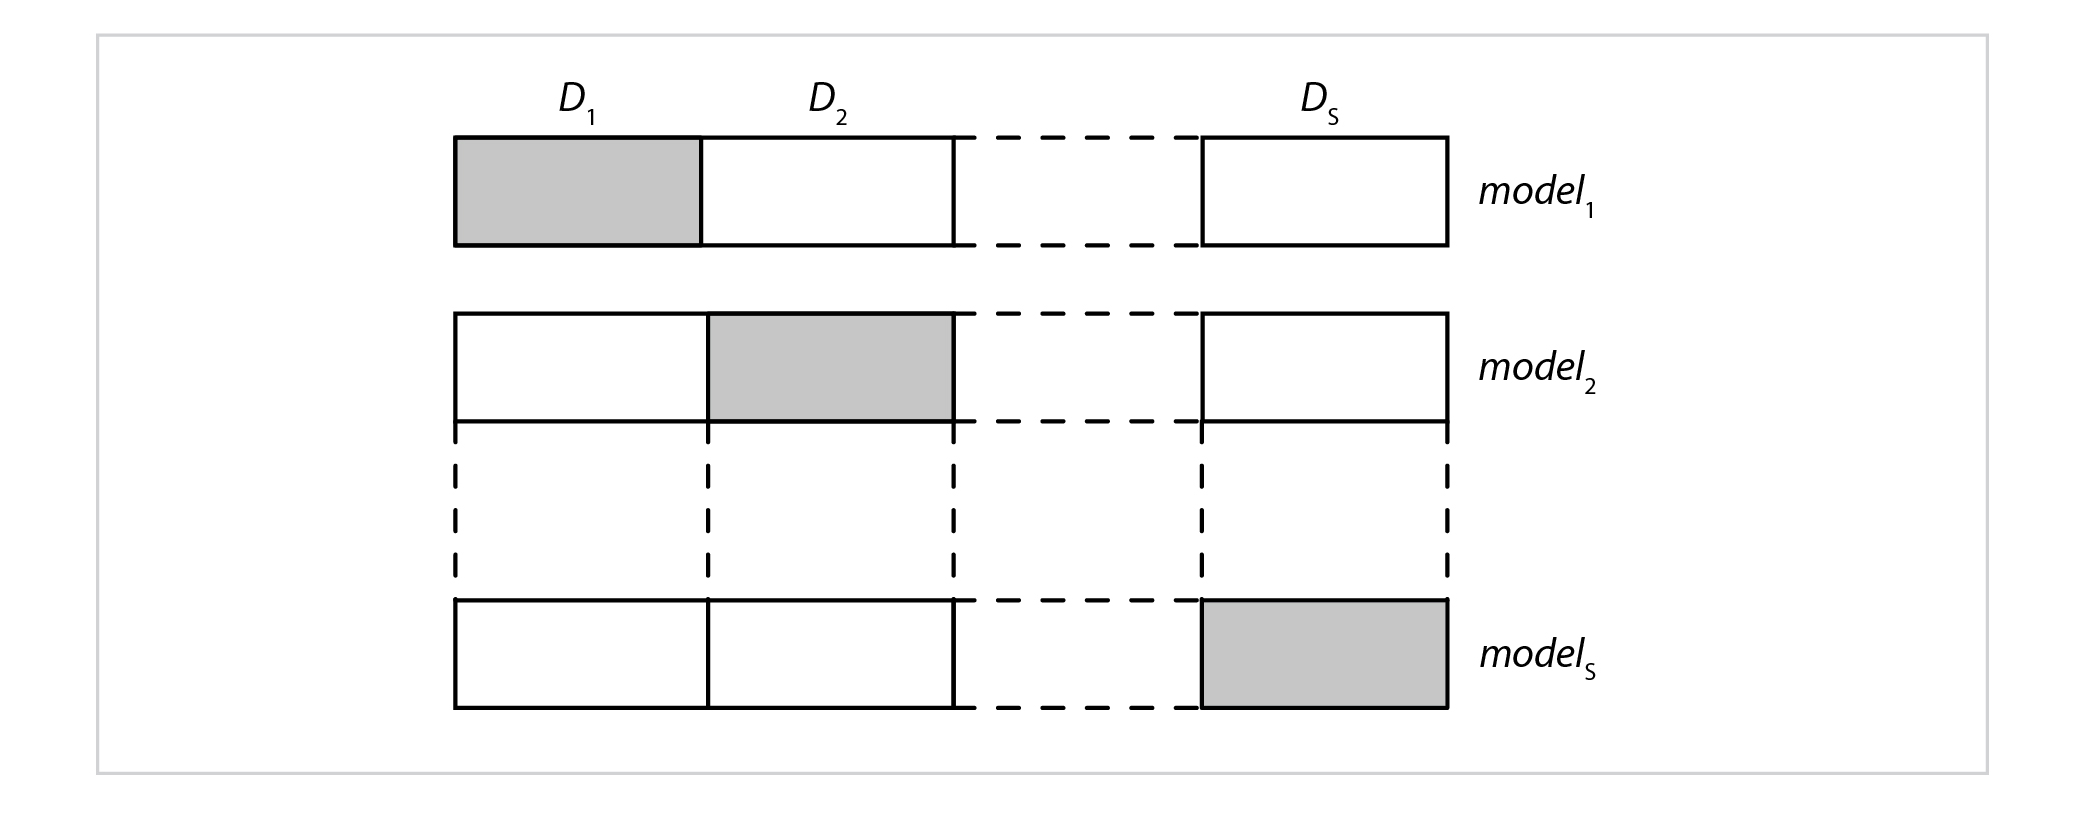
\includegraphics[width=0.55\textwidth]{figures/cross-validation.png}
	\caption{Reprezentacja graficzna oceny krzyżowej.}
	\label{cross-validation}
\end{figure}

Stosując metodę oceny krzyżowej dla różnych modeli sieci można stwierdzić, który z nich spełnia najlepiej kompromis między dobrą klasyfikacją zbioru $U$ i wysoką generalizacją.

Kombinacja predykcji wielu różnych modeli jest bardzo wydajną metodą do polepszenia generalizacji i zmniejszenia błędu klasyfikacji na zbiorach testowych oraz walidacyjnych (zob. [AlexNet 1, 3]). Jednak współczesne sieci neuronowe, których przykłady zostały opisane w dalszych sekcjach mogą zawierać miliony parametrów, których optymalizacja jest wymagająca obliczeniowo. Z uwagi na ten fakt trening $s$ segmentów jest mało wydajny i stosuje się go w ograniczonym zakresie np. obierając $s$ = 5 lub $s$ = 10.

W 2012, w [AlexNet-10] zaproponowano technikę zwaną \textit{dropout}, której główna idea bazuje na zerowaniu wyjścia neuronów sieci z prawdopodobieństwem 0,5 przy każdej iteracji treningu sieci. Neurony, które są w ten sposób tymczasowo dezaktywowane nie mają wpływu w danej iteracji na predykcję sieci i nie są uwzględniane przy wstecznej propagacji gradientu. Podejście to można porównać do treningu w każdej iteracji różnych modeli sieci. Dla przykładu w [AlexNet] wykazano, że metoda dropout wymaga jedynie 2 razy więcej iteracji do przybliżenia zbioru $U$, przy tym uzyskuje znacznie lepszą generalizację. 

Kluczowym składnikiem potrzebnym do treningu sieci i maksymalizacji generalizacji jest odpowiedni rozmiar zbioru danych. W praktyce jest to problem szeroko dyskutowany, gdyż zwłaszcza w danych medycznych istnieje szereg ograniczeń związanych z dostępem i akwizycją odpowiedniego materiału badawczego (np. ograniczenia: prawne, związane z prywatnością, czy z etyką). W przypadku, gdy zgromadzenie odpowiedniego zbioru danych jest niemożliwe pewnym rozwiązaniem problemu jest zastosowanie metod jego sztuczego powiększania (ang. \textit{data augmentation}).

W przypadku obrazów stosuje się metody afinicznych przekształceń. Są to najczęściej rotacje, odbicia lub skalowanie. W określonych przypadkach używane są również nielioowe przekształcenia. Np. w [Ronneberger et al., arXiv:1505.04597v1, 2015] wykorzystano m.in. deformacje do powiększenia zbioru 30 obrazów mikroskopowych przedstawiających macierz komórkową i uzyskano znacząco lepsze wyniki niż istniejące w 2015 algorytmy typu state-of-the-art.

W przypadku danych medycznych należy szczególnie zwrócić uwagę, aby powiększony zbiór zawierał dane przypominające w rzeczywistości występujące przypadki np. nieduże obroty występujące u pacjentów skanowanych rezonansem magnetycznym lub niewielkie skalowania rozmiaru organów. Szeroką dyskusję prowadzi się również na temat wykorzystania sztucznie generowanych zbiorów danych o czym więcej można przeczytać w pracach [Sztuczna generacja danych medycznych]. 


\subsection{Problem redukcji wymiarowości}

Rozmiar wektora cech wejściowych we współczesnych problemach rozwiązywanych przez algorytmy sztucznej inteligencji często osiąga liczby liczone w tysiącach (zob. [przykłądy dużych problemów FB, Google]). Również w powszechnie używanych głębokich sieciach neuronowych ekstraktor cech tworzy wektor o rozmiarach tego rzędu.

Duży rozmiar wektora cech wejściowych prowadzi do problemu nazwanego \textit{przekleństwem wymiarowości} (ang. \textit{curse of dimensionality}). Określenie te zostało poraz pierwszy sformułowane przez Richarda Bellmana w latach 50-tych XX wieku. Naukowca zajmującego się teorią sterowania (zob. [teoria sterowania]), który podczas swojej pracy obserwował algorytmy doskonale działające w 3 wymiarach, a prezentujące znacząco gorsze wyniki w hiperprzestrzeni. 

Problemy z zastosowaniem algorytmów szucznej inteligencji w tym głębokich sieci neuronowych w dużej liczbie wymiarów mają dwie główne przyczyny: (1) w miarę wzrostu liczby wymiarów cech liczba obserwacji w zbiorze trenującym potrzebnych do wiarygodnego oszacowania funkcji wyjściowej rośnie wykładniczo; (2) nie wszystkie cechy są jednakowo znaczące w kontekście rozróżnienia danych.  

Problem (2) jest szczególnie istotny w dość prostych algorytmach takich jak algorytm K najbliższych sąsiadów, gdzie do poprawnego działania należy policzyć dystans pomiędzy sąsiednimi obserwacjami. Uwzględniając dużą liczbę nieistotnych cech jako argumenty funkcji dystansu uzyskuje się wyniki uniemożliwiające poprawną klasyfikację zbioru. 

W przypadku głębokich sieci neuronowych zastosowanie wag zmniejsza znaczenie problemu (2), gdyż wpływ poszczególnych cech może być regulowany poprzez wartość $w$. W przypadku problemu wynikającego z (1) można wyróżnić dwa podejścia stosowane do jego niwelacji:
\begin{itemize}
\item wybór podzbioru istotnych cech o liczności $n'$ $<<$ $n$,
\item przekształcenie oryginalnych $n$ zmiennych na nowy zbiór $n'$ cech, gdzie ponownie $n'$ $<<$ $n$.

\end{itemize}

/*rozwinąć i wprowadzić definicję korelacji oraz entropii - zapytać Kubę jakby ten akapit widział*/

Wybór podzbioru istotnych cech polega na określeniu minimalnego podzbioru, dla którego rozkład prawdopodobieństwa różnych klas obiektów jest jak najbliższy oryginalnemu rozkładowi uzyskanemu z wykorzystaniem wszystkich cech. W tym celu stosuje się np.: miary siły związku [], testy wykorzystujące entropię względną [], badania korelacji wzajemnych [], teorię zbiorów przybliżonych [] itp.

W kontekście przekształcenia zbioru cech najczęściej wykorzystywaną metodą jest algorytm \textit{analizy składowych głównych} ) (ang. \textit{Principal Component Analysis}, w skr. PCA) opracowany przez Karla Pearsona w 1901 r (zob. Pearson1901).  
Istotą PCA jest ortogonalne przekształcenie początkowych skorelowanych cech w nowy zbiór nieskorelowanych zmiennych. Każdy z nowych wektorów jest kombinacją liniową pewnych
składowych głównych (odnoszących się do oryginalnych cech). Nowe nieskorelowane zmienne, tzw. \textit{składowe główne}, powstają z przekształcenia oryginalnych zmiennych skorelowanych, w taki sposób aby w maksymalnym stopniu wyjaśniać całkowitą wariancję w próbie cech oryginalnych. Wariancje składowych głównych są wartościami własnymi macierzy kowariancji oryginalnych zmiennych. Dla przykładu pierwsza składowa główna redukuje największą część zróżnicowania, druga kolejną której nie redukowała poprzednia itp.

Procedure PCA można zapisać następująco:
\begin{enumerate}
\item oblicz macierz kowariancji: Sx = $X^{T}X$, gdzie $X$ to macierz danych zawierająca obserwacje w wierszach. macierz Sx jest symetryczna i pozwala ocenić: (1) wariancje zmiennych (elementy na głównej przekątnej); (2) zależności pomiędzy zmiennymi (elementy poza główną przekątną) 
\item dokonaj rozkładu: Sx = $KLK^T$
\item utwórz nowe zmienne wykonując operację: Y = XK
\end{enumerate}
/*przykład numeryczny https://www.itl.nist.gov/div898/handbook/pmc/section5/pmc552.htm */

Oprócz PCA można również wyróznić nastepujące algorytmy: 
\begin{enumerate}
	\item t-SNE
	\item ISOMAP: Isomap Homepage 
	\item ICA: What is Independent Component Analysis ?
	\item LSA: Popular in NLP domain :: LSA @ CU Boulder
	\item Sammon mapping: Implementation in python tompollard/sammon
	\item Self Organizing Maps: Matlab implementation SOM Toolbox	
	
	https://www.quora.com/What-are-different-unsupervised-feature-selection-methods-other-than-principle-component-analysis-PCA
\end{enumerate}




\section{Przykłady współczesnych topologii}

/*co pozwoliło na obliczenia NVIDIA, TPU, RAM, Google Brain i głębokość obecnych sieci*/

\subsection{AlexNet}
\label{AlexNet}
Sieć AlexNet, której nazwa pochodzi od imienia głównego twórcy tej architektury Alexa Krizhevsky, zawiera blisko 60 milionów parametrów i 650 tysięcy neuronów. Architekturę zaprezentowano na Rys. \ref{AlexNetTopology}
\begin{figure}[h!]
	\centering
	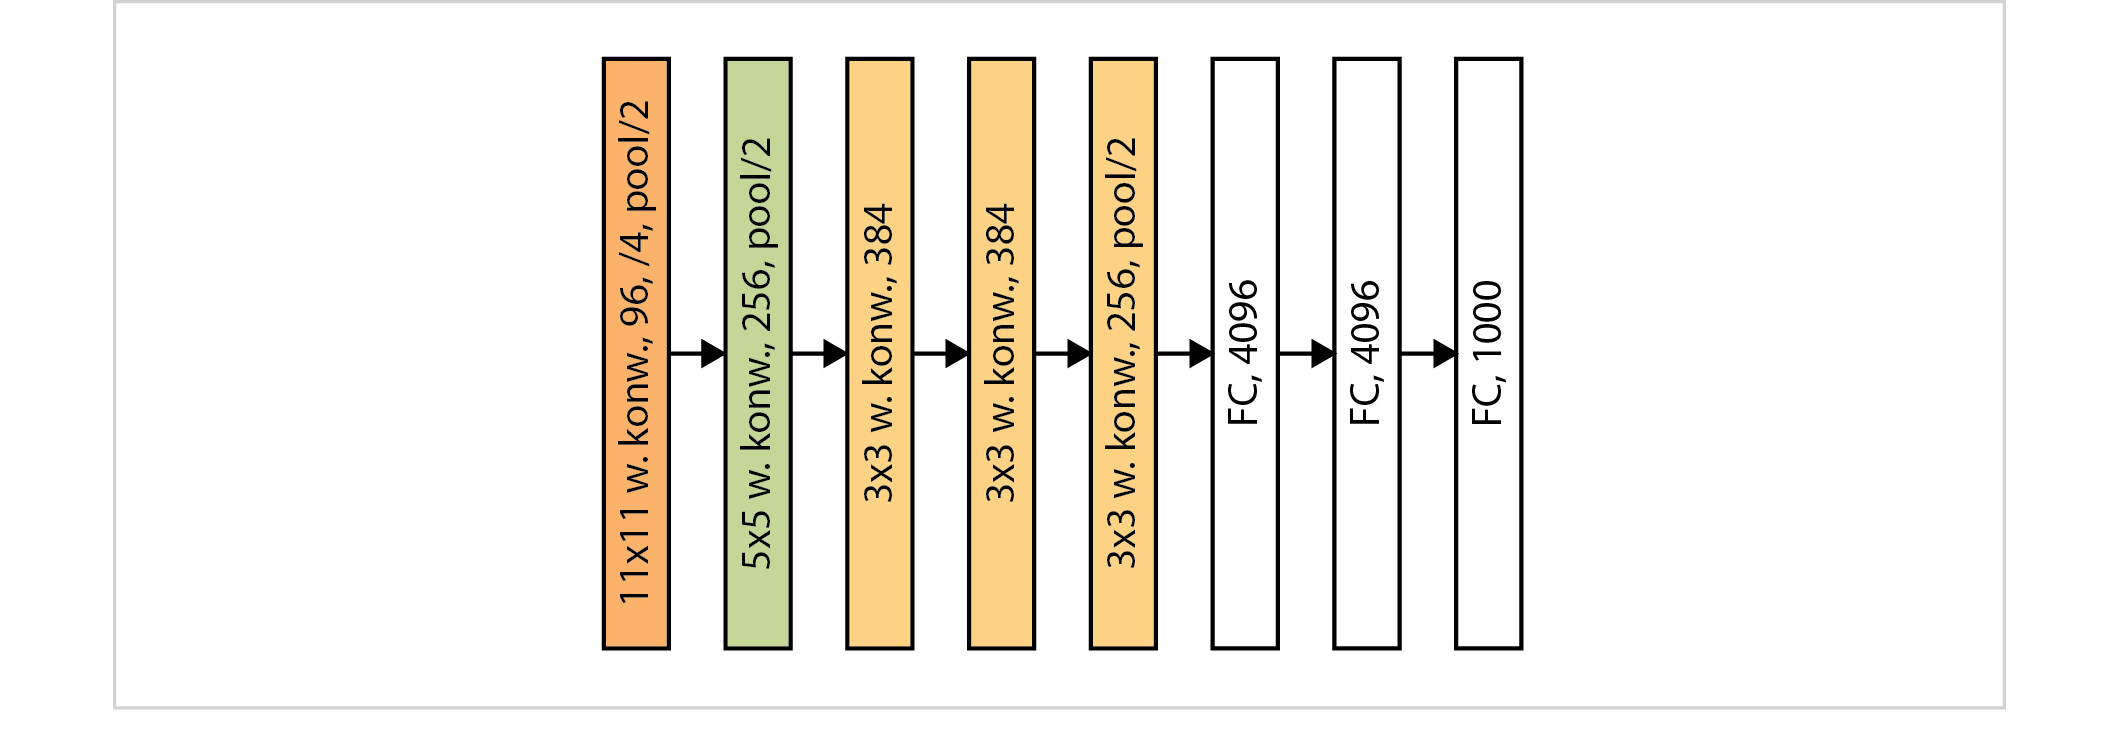
\includegraphics[width=0.55\textwidth]{figures/AlexNet.png}
	\caption{Topologia architektury AlexNet.}
	\label{AlexNetTopology}
\end{figure}

W skład topologii wchodzi pięć warstw konwolucyjnych i trzy typu fully-connected. Po pierwszej, drugiej i piątej warstwie konwolucyjnej występują operacje typu max-pool z jądrem o wymiarach 2$\times$2 \footnote{autorzy pracy podają też przykłady użycia jąder o wymiarze 2$\times$3, które nakładają się w przestrzeni funkcji obrazowej}. 

Pierwsza warstwa konwolucyjna przyjmuje na wejściu dane o wymiarze 227$\times$227$\times$3, na których wykonywana jest operacja splotu z 96 filtrami z jądrem splotu o wymiarach 11$\times$11$\times$3 i krokiem 4. W rezultacie (uwzględniając również operację max-pool) objętość wynikowa przekazywana do kolejnej warstwy ma wymiar 27$\times$27$\times$96. W drugiej warstwie konwolucyjnej wykonywana jest operacja splotu z 256 filtrami z jądrem o wymiarach 5$\times$5$\times$96. Wymiar objętości wynikowej zostaje ponownie zredukowany poprzez operacje max-pool do 13$\times$13$\times$256. Kolejne 3 warstwy konwolucyjne są połączone bezpośrednio ze sobą. Trzecia warstwa zawieraja 384 filtry o wymiarze 3$\times$3$\times$256, w skład czwartej wchodzą 384 filtry o wymiarze 3$\times$3$\times$384, a w piątej znajdują się 256 filtry ponownie o wymiarze 3$\times$3$\times$384. Końcowe dwie warstwy typu FC zawierają po 4096 neuronów, a ostatnia zawiera tyle neuronów ile klas występuje w ostatecznym podziale - w oryginalnej pracy było to 1000 [AlexNet].

W celu lepszego zrozumienia przetwarzania sygnału wejściowego przez sieć poniżej przedstawiono przykład algorytmu wykorzystywanego dla pierwszej warstwy konwolucyjnej opisywanej topologii: 
\begin{enumerate}
\item Z danych wejściowych o wymiarze [227$\times$227$\times$3] wybierany jest co czwarty blok (zarówno wzdłuż wysokości jak i szerokości) o wymiarach [11$\times$11$\times$3]. Punkty krawędziowe, które stanowią margines potrzebny do wyliczenia splotu są zazwyczaj pomijane. W rezultacie otrzymywanych jest 217 punktów w każdym rzędzie i w kolumnie, w których mieści się [55$\times$55] tj. 3025 bloków.
\item Zarówno 11$\times$11$\times$3 = 363 wagi znajdujące się w 96 filtrach jak i wartości 363 punktów obrazowych znajdujących sie 3025 blokach są przedstawiane w postaci macierzy $A$ o wymiarach [96$\times$363] i $B$ o wymiarach [363$\times$3025].
\item liczony jest iloczyn skalarny w postaci A$^\intercal$B = $C$, gdzie nowa, wyjściowa macierz $C$ ma wymiar [96$\times$3025].
\item Resultat w postaci macierzy $C$ ponownie przewymiarowywany jest na postać [55$\times$55$\times$96].  
\end{enumerate} 

W architekturze jako funkcję aktywacji neuronów wykorzystano ReLU, co znacząco przyspieszyło trening sieci. Dla przykładu uzyskano 6-krotne przyspieszenie treningu dla danych CIFAR-10 [CIFAR] w stosunku do tej samej topologii wykorzystującej funkcję aktywacji tanh.

Ponieważ funkcja ReLU nie posiada górnego ograniczenia neurony teoretycznie mogą posiadać nieograniczone wartości funkcji aktywacji. W celu polepszenia kontrastu pomiędzy neuronami i wydobycia tych, które na tle innych się wyróżniają, zastosowano normalizację:
\begin{equation}
b^i_{x,y} = a^i_{x,y}/\left ( k + \alpha \sum_{j=max(0,i-n/2)}^{min(N-1,i+n/2)} (a^i_{x,y})^2 \right  )^\beta 
\label{AlexNetNorm}
\end{equation}
gdzie $n$ to liczba filtrów znajdujących się w tej samej przestrzennej lokalizacji, $N$ to suma wszystkich filtrów w warstwie, $a^i_{x,y}$ to wartość funkcji aktywacji neuronu po splocie funkcji obrazowej na pozycji ($x$, $y$) z filtrem $i$, a $b$ to wynik normalizacji. Po zastosowaniu tej techniki autorom pracy udało się zredukować błąd klasyfikacji top-5 o wartość 1,2 punkta procentowego.

W kontekście zwiększenia efektywności treningu zastosowano powiększenie rozmiaru danych poprzez rotacje i modyfikacje funkcji obrazowej z wykorzystaniem czynników głównych (zob [AlexNet]), co zmniejszyło błąd top-1 o 1\%. Zastosowano również technikę dropout opisaną w \ref{sec-overffiting}. Ostatecznie wprowadzono także trening z wykorzystaniem wielu GPU (zob. Rys. \ref{AlexNetTopologyMultiGPU}). 

\begin{figure}[h!]
	\centering
	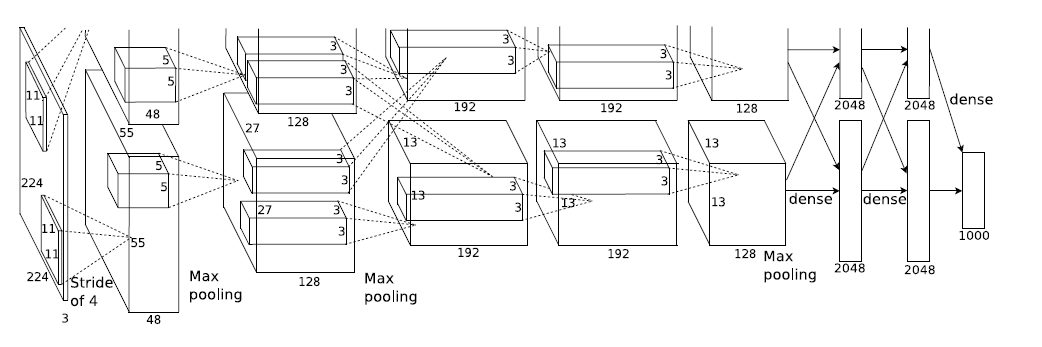
\includegraphics[width=0.8\textwidth]{figures/AlexNet-multiGPU.png}
	\caption{Topologia architektury AlexNet z podziałem na dwa akceleratory GPU.}
	\label{AlexNetTopologyMultiGPU}
\end{figure}

Topologia z podziałem na 2 karty zwiększyła dwukrotnie sumaryczną pamięć i pozwoliła na koalokację parametrów sieci.

Praca Alexa Krizhevsky, Ilya Sutskever i Geoffrey'a Hinton zapoczątkowała wzrost zainteresowania technikami głębokiego uczenia się, co doprowadziło do publikacji kolejnych podobnych architektur. Do najbardziej znanych należą ZFNet z 2013 roku [ZFNet], gdzie m.in. zastosowano zmniejszenie wymiaru jądra stosowanego w filtrach pierwszej warstwy konwolucyjnej do 7$\times$7 oraz VGGNet z 2014 roku, gdzie zastosowano większą liczbę warstw konwolucyjnych z mniejszym wymiarem jądra splotu. Innowacyjnym pomysłym, który został zaprezentowany również w 2014 było pojawienie się nowych modułów w sieci GoogleNet, która dokładniej została opisana w kolejnej podsekcji.

\subsection{GoogLeNet}

Architekturę o nazwie GoogLeNet zaprezentowano w 2014 r. w pracy [GoogleNet]. Nazwa architektury pochodzi od nazwy zwycięzkiego zespołu startującego w ILSVRC14, składającego się z pracowników firmy Google. Oryginalnie topologia składała się z 22 warstw i zawierała około 5 mln parametrów (12 razy mniej niż w przypadku sieci AlexNet). 

Redukcję liczby parametrów przy jednoczesnym podwyższeniu dokładności klasyfikacji i lokalizacji obiektów (zob. [ILSCV]) udało się uzyskać poprzez poszukiwania konstrukcji optymalnych lokalnych topologii i ich połączeń. Mianowicie, wiadomo że duża część funkcji aktywacji neuronów przyjmuje wartość 0 lub jest redundatna z powodu wysokiej korelacji między sobą (zob. [Arora z GoogleNet]). Matematyka dotycząca przetwarzania \textit{macierzy rzadkich}, tj. gdzie przeważająca liczba elementów przyjmuje wartość 0, jest dobrze znana np. [3-GoogleNet]. Jednak implementacje bibliotek do obliczeń związanych z algebrą liniową są zooptymalizowane pod kątem \textit{macierzy gęstych}, gdzie przeważająca liczba elementów przyjmuje wartości różne od 0 (zob. [16, 9 googleNet]). 

Ideą modułu incepcji zaproponowanego przez twórców GoogLeNet jest aproksymacja rzadkich macierzy z użyciem komponentów o gęstej strukturze. Takie komponenty nazwano \textit{modułami incepcji} (ang. \textit{inception modules}). Przykłądy modułów incepcji pokazano na Rys. \ref{GoogleNetInceptionModules} 
\begin{figure}[h!]
	\centering
	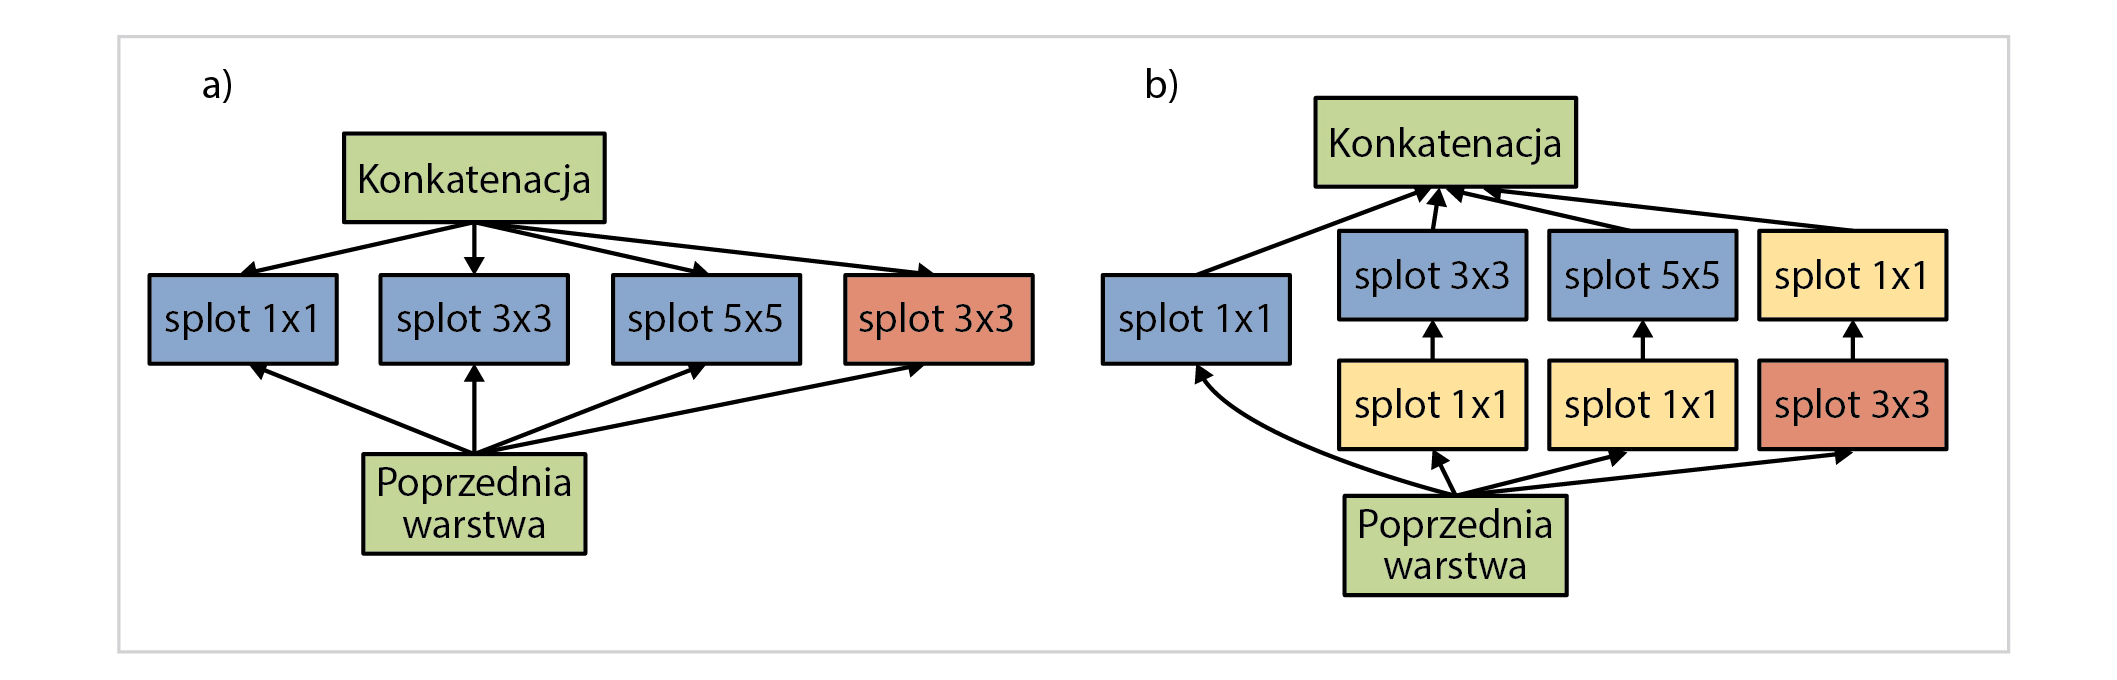
\includegraphics[width=0.8\textwidth]{figures/InceptionModules.png}
	\caption{Topologia architektury AlexNet z podziałem na dwa akceleratory GPU.}
	\label{GoogleNetInceptionModules}
\end{figure}

Rys. \ref{GoogleNetInceptionModules} (a) przedstawia najwną formę modułu incepcji, gdzie grupowane są operacje filtrów z jądrem o wymiarach 5$\times$5, 3$\times$3, 1$\times$1 oraz operacja max-pool. Rys. \ref{GoogleNetInceptionModules} (b) prezentuje koncepcję zooptymalizowaną obliczeniowo gdzie filtry 1$\times$1 służą do redukcji wymiarowości i używane są bezpośrednio przed splotami z bardziej wymagającymi obliczeniowo splotami z jądrami o wymiarach 5$\times$5 i 3$\times$3. 

Złożenie różnego rodzaju modułów dało topologię zaprezentowaną na Rys.
\begin{figure}[h!]
	\centering
	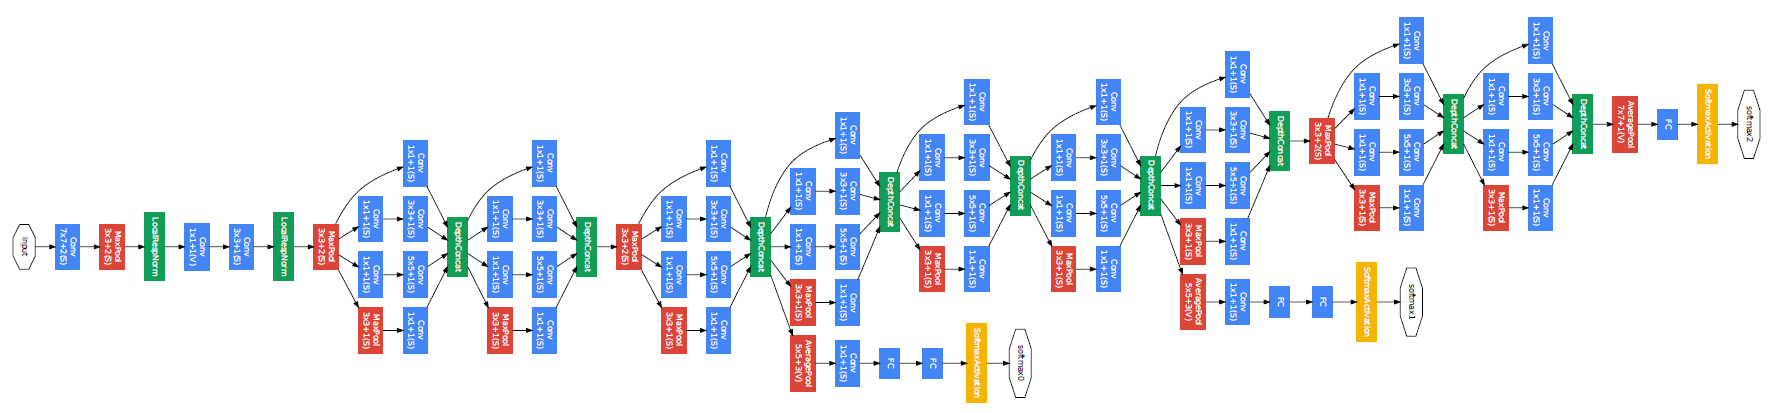
\includegraphics[width=1\textwidth]{figures/GoogleNet.png}
	\caption{Topologia architektury GoogleNet}
	\label{GoogleNetTopo}
\end{figure}

Dokładne zestawienie parametrów znajduje się w Tabeli \ref{GoogleNetParams}

\begin{table}[h!]
	\centering
	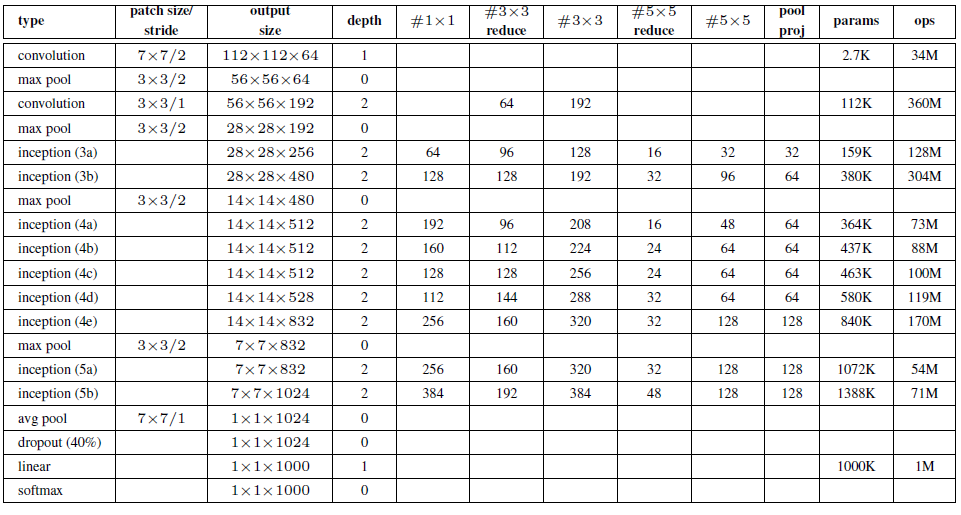
\includegraphics[width=1\textwidth]{figures/GoogleNetparams.png}
	\caption{Parametry architektury GoogleNet}
	\label{GoogleNetParams}
\end{table}

Ważną cechą sieci GoogleNet jest brak warstw typu FC na zakończeniu, gdzie w przypadku sieci AlexNet znajdowało się około 90\% parametrów. Końcowe wnioskowanie jest realizowane na podstawie wartości średniej z dwuwymiarowych map cech.

Dla lepszego zrozumienia idei redukcji wymiarowości realizowanej przez moduły incepcji, podobnie jak w przypadku sieci AlexNet, przeanalizowane zostanie działanie pierwszego modułu w topologii z Rys. \ref{GoogleNetTopo}.
Moduł zawiera 128 filtrów z jądrami o wymiarach 3$\times$3 i 32 filtry z jądrami o wymiarach 5$\times$5. Dane na wejściu modułu mają 192 kanały (zob. Tabela \ref{GoogleNetParams}). Dla przykładu, rząd wielkości obliczeń operacji splotów 32 filtrów 5$\times$5 wynosi 25$\times$32$\times$192=153 600 i dalej wzrastałby z głębokością sieci. W celu zapobiegnięcia nadmiarowi obliczeń stosowana jest redukcja z użyciem 16 filtrów z jądrem o wymiarach 1$\times$1. W efekcie rząd wielkości obliczeń spada do 16$\times$192 +  25$\times$32$\times$16=15 876, co pozwala na dalsze budowanie wielowarstwowych struktur.

Topologia GoogLeNet jest wciąż rozwijana. Po pierwszej prezentacji pojawiły się kolejne modernizacje wprowadzjące dodatkowe faktoryzacje modułów jak w Inception-v2 [Inception-v2], lub normalizacje wartości wynikowych poszczególnych warstw jak w Inception-v3 [Inception-v3]. Kolejny innowacyjny pomysł, bazujący na dodatkowych połączeniach między blokami, został wprowadzony w 2015 roku w sieci ResNet, która została opisana w kolejnej podsekcji.

\subsection{ResNet}

Jednym z najbardziej oczywistych pomysłów na polepszenie dokładności działania sieci neuronowych jest zwiększenie liczby warstw. Jednak wraz ze wzrostem liczby warstw, trening takich architektur z użyciem tradycyjnych metod gradientowych (takich jak algorytm wstecznej propagacji błędu) staje się mniej wydajny. Problem wynika z faktu, że zmiana wartości sygnału na wyjściu sieci w odpowiedzi na sygnał wejściowy jest mniejsza wraz ze wzrostem liczby warstw [ResNet]. W takiej sytuacji gradient wyliczany na podstawie sygnału będącego różnicą pomiędzy sygnałem wejściowym a wejściowym może przyjmować wartości bliskie 0 uniemożliwiając progres uczenia się. Problem zanikającego gradientu (ang. \textit{vanishing gradient problem}) rozwiązywany jest poprzez zastosowanie normalizacji oraz nieliniowych funkcji aktywacji, których przykłady zostały opisane w sekcji \ref{AlexNet} oraz szeroko w literaturze np. w [ResNet 2,3,4]. Dzięki tym mechanizmom algorytm treningu głębokich sieci neuronowych w większej liczbie przypadków zbiega do użytecznego minimum lokalnego. 

W momencie znalezienia takiego minimum dodanie kolejnych warstw i parametrów sieci jest redundatne, a nawet prowadzi do pogorszenia wyników treningu sieci, co związane jest z trudnościami optymalizacji przestrzeni wieloparametrycznych [Opt]. Zjawiskio to nosi nazwę degradacji treningu (ang. \textit{degradation problem}). Twórcy architektury ResNet zaproponowali rozwiązanie tego problemu poprzez implementację bloków rezydualnych (ang. \textit{Residuum Units}) zawierających dodatkowe, skrótowe połączenia (ang. \textit{skip conections}) pomiędzy wejściem a wyjściem bloków. Porównanie schematów funkcjonalnych nowych bloków i wcześniej istniejącego rozwiązania stosowanego np. w AlexNet został przedstawiony na Rys. \ref{ResNetBlock}.
\begin{figure}[h!]
	\centering
	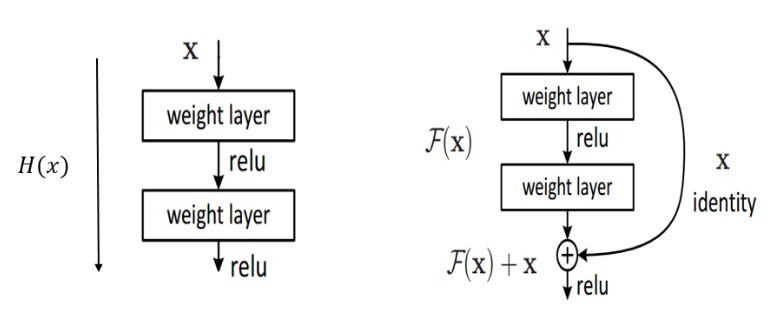
\includegraphics[width=0.5\textwidth]{figures/ResidualBlock.jpg}
	\caption{Schemat funkcjonalny pojedynczego bloku w architekturze ResNet.}
	\label{ResNetBlock}
\end{figure} 

Ogólną postać równania bloku rezydualnego można zapisać następująco:
\begin{equation}
\begin{split}
y_l = h(x_l) + F(x_l, W_l),\\
x_{l+1} = f(y_l),
\end{split}
\end{equation}
gdzie $x_l$ i $x_{l+1}$ stanowią sygnał wejściowy i wyjściowy $l$-tego bloku. $F$ stanowi funkcję rezydualną optymalizowaną podczas treningu sieci, $h$($x_l$) stanowi funkcję przekształcenia sygnału $x_l$ przekazywanego skrótowym połączeniem, $f$ jest funkcją ReLU, a $W$ stanowi macierz wag.

Funkcja $h$($x_l$) jest funkcją tożsamościową, a zatem $h$($x_l$) = $x_l$. Żeby uzasadnić ten wybór należy rozważyć propagację gradientu wewnątrz sieci skłądającej się z bloków rezydualnych. Dla każdego $L$-tego bloku zachodzi równanie:
\begin{equation}
x_L = x_l + \sum_{i=l}^{L-1}F(x_i, W_i)
\end{equation}
Korzystając z reguły łąńcuchowej [ResNet-wyj-9] można zapisać równanie na gradient funkcji kosztu $\varepsilon$:
\begin{equation}
\ref{gradResBlock}
\frac{\partial \varepsilon}{\partial x} =  \frac{\partial \varepsilon}{\partial x_L} \frac{\partial x_L}{\partial x_l} =  \frac{\partial \varepsilon}{\partial x_L}\left (1 +   \frac{\partial }{\partial x_l}\sum_{i=l}^{L-1}F(x_i, W_i) \right )
\end{equation}
z czego wynika, że gradient może być podzielony na dwie addytywne składowe: (1) $w$ = $\frac{\partial \varepsilon}{\partial x_L}$ propagowaną bez wpływu na warstwy zawierające wagi i (2) $\lambda$ = $\frac{\partial \varepsilon}{\partial x_L}\frac{\partial }{\partial x_l}\sum_{i=l}^{L-1}F(x_i, W_i)$ propagowaną przez nie.

Przykład propagacji gradientu w sieci składającej się z trzech bloków wyglądałby następująco:
\begin{equation}
\frac{\partial \varepsilon}{\partial x_0} =  \frac{\partial \varepsilon}{\partial x_3}*(w_2+\lambda_2)*(w_1+\lambda_1)*(w_0+\lambda_0)
\end{equation}

Przyjmując, że wartości $w$ są zazwyczaj znormalizowane do przedziału (-1;1) można rozważyć 4 istotne przypadki:
\begin{enumerate}
	\item $\lambda$ = 0 -- nie ma skrótowych połączeń, co odpowiada płaskiej strukturze sieci. Ponieważ wartości $w$ są z przedziału (-1;1) dodawanie kolejnych warstw wzmacnia wcześniej omówiony efekt zanikającego gradietu.
	\item $\lambda$ $>$ 1 -- z każdą warstwą, sumaryczna wartość gradientu zwiększa się inkrementalnie, co nazywane jest \textit{problemem eksplozji gradientu} (ang. \textit{exploding gradient problem}).
	\item $\lambda$ $<$ 1 -- przy założeniu, że $w$ + $\lambda$ $<$ 1, dla sieci skłądających się z wielu warstw występuje problem zaniku gradientu, jak w przypadku 1. Natomiast, gdy $w$ + $\lambda$ $>$ 1 podobnie jak w przypadku 2 może występować problem eksplozji gradienu.
	\item $\lambda$ $=$ 1 -- wartości $w$ są inkrementowane dokładnie o 1, co eliminuje problemy podane w przypadkach 1, 2 i 3 i stanowiło motywacje dla twórców architektury ResNet dla wyboru funkcji tożsamościowej $h$($x_l$).
\end{enumerate}

Dokładny opis matematyczny funkcjonowania bloków rezydualnych wraz z dowodami znajduje się w [ResNet-wyj]. Przykład topologii sieci składającej się z 8 bloków i łącznie 18 warstw tzw. ResNet-18, przedstawiono na Rys.
\begin{figure}[h!]
	\centering
	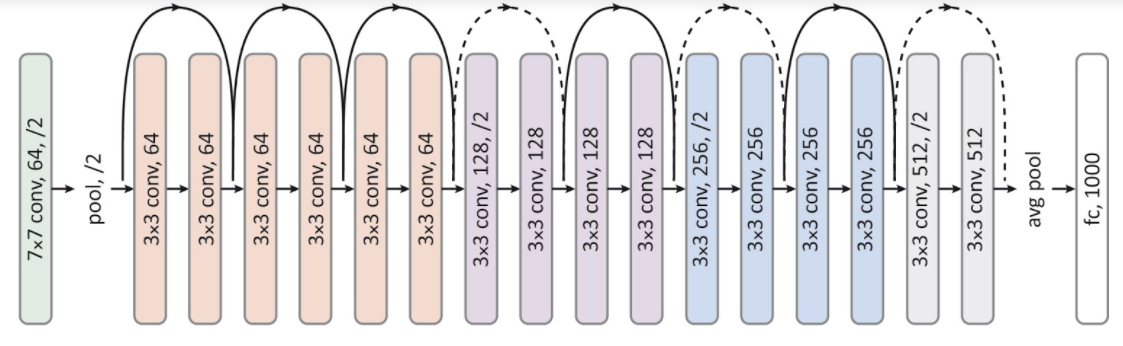
\includegraphics[width=1\textwidth]{figures/ResNet.png}
	\caption{Topologia architektury ResNet-18.}
	\label{ResNetBlock}
\end{figure} 

Pierwsza warstwa konwolucyjna zawiera filtry z jądrem splotu o wymiarach 7$\times$7. W kolejnych zastosowano wymiar 3$\times$3. Zastosowanie mniejszych wymiarów jąder splotu niż w AlexNet oraz podobnie jak w przypadku sieci GoogLeNet wyliczenie na końcu wartości średniej z dwuwymiarowych map cech zredukowało liczbę parametrów.

Architektura ResNet-18 jest najmniejszą z pojawiających się w literaturze przykładów. W praktyce, z powodzeniem wykorzystywano topologie składające się nawet z 1202 warstw [ResNet]. W 2016 roku zaprezentowano hybrydę sieci GoogleNet i ResNet [InceptionResNet]. Pracowano również nad bardziej złożonymi blokami, co w konsekwencji doporwadziło w 2017 roku do zaprezentowania architektury ResNetX, która w wielu testach klasyfikacji różnych zbiorów okazała się być lepsza niż poprzednicy [ResNetX]. Ciekawy przegląd dotyczący historii tych prac można znaleźć w [https://towardsdatascience.com/an-overview-of-resnet-and-its-variants-5281e2f56035].

Sieć ResNet i jej warianty dla wielu testowych zbiorów danych takich jak ImageNet, CIFAR czy COCO osiągneły dokładność klasyfikacji porównywalną z możliwościami ludzkiego obserwatora. Dalszy progres był możliwy m.in. dzięki zastosowaniu synergii wielu modeli, co zostało opisane w kolejnej podsekcji.

\subsection{Złożenia}
Uczenie złożeń sieci (ang. \textit{esemble learning}) polega na wykorzystywaniu kilku modeli bazowych i wybranej metody ich synergii. Koncepcja nie jest nowa i stosowana była już przed etapem kiedy to metody głębokiego uczenia się zyskały na popularności. Dobry przegląd wcześniejszych prac bazujących na tradycyjnym podejściu do uczenia maszynowego można znaleźć w  [Ensemble 1-3].

W kontekście głębokiego uczenia się stosowane są różnea metody kombinacji modeli bazowych [Ensemble]. Jako często stosowane przykłady można podać: uśrednianie, głosowanie, klasyfikacja Bayesa, generalizację stosów. Zostaną one omówione w kolejnych paragrafach:

\subsubsection{Uśrednianie}
Uśrednianie jest prostą metodą kombinacji wyników predykcji. Najczęściej stosowane jest uśrednianie bez wag, gdzie suma wyników predykcji modeli bazowych podzielona jest przez liczbę tych modeli. Uśredniać można bezpośrednio wyniki finalnej predykcji jak również prawdopodobieństwa przynależności do odpowiednich klas, które są np. wynikiem funkcji softmax. 

Główną zaletą uśredniania jest redukcja wariancji. Jest ona tym większa im bardziej nieskorelowane są wyniki predykcji modeli bazowych. Pomimo prostoty tego rodzaju koncepcja odnosiła już sukcesy m.in. w lasach losowych (Breiman, 2001).

Zastosowanie uśredniania przy silnie odstających od średniej najgorszych predykcjach znacząco obniża dokładność całego złożenia. Dlatego przy silnie nieheterogenicznych modelach bazowych dających bardzo różne wyniki często poszukiwane są inne metody.

\subsubsection{Głosowanie}

W głosowaniu stosuje się mechanizm zliczania przewidzianych przez modele bazowe etykiet. Etykieta, która została wybrana przez największą liczbę modeli bazowych jest obierana jako wynik ostatecznej predykcji. Jest to tzw. \textit{głosowanie większościowe}.

W porównaniu do uśredniania, głosowanie jest mniej czułe na predykcje pojedynczych modeli. Wykorzystuje jednak jedynie informacje o przewidzianych etykietach, co utrudnia konstrukcje bardziej wyszukanych rozwiązań.

\subsubsection{Klasyfikacja Bayesa}

W przypadku tej metody, każdy model bazowy $j$ postrzegany jest jako hipoteza $h_j$. Każda z hipotez posiada wagę proporcjonalną do prawdopodobieństwa zdarzenia, w którym dany zbiór danych trenujących zostałby wybrany z ogółu danych gdyby dana hipoteza była prawdziwa. Jest to tzw. optymalna klasyfikacja Bayesa, którą można zapisać następującycm równaniem:
\begin{equation}
y = armax_{c_j \in C} \sum_{h_i \in H} P(c_j \mid h_i)P(T \mid h_i)P(h_i)
\end{equation}
gdzie $y$ to przewidziana etykieta, $C$ jest zbiorem wszystkich możliwych klas, $H$ to przestrzeń hipotez, a $T$ to zbiór danych trenujących.

W praktyce z uwagi na dużą złożoność obliczeniową optymalną klasyfikację Bayesa wykorzystuje się rzadko. Cześćiej stosowane są techniki BPA (od ang. \textit{Bayesian parameter averaging}), BMA (od ang. \textit{Bayesian model averaging}), czy teć BMC (od ang. \textit{Bayesian model combination}) (zob. [BPA, BMA, BMC]), które aproksymują optymalną metodę.

\subsubsection{Generalizacja stosów}
Idea generalizacji stosów oryginalnie została zaproponowana w [Wolpert, 1992]. Wykorzystana została koncepcja meta-uczenia, a zatem konstrukcja nadrzędnego klasyfikatora, którego zadniem jest wybór optymalnego wektora wag $a$ dla stosu $s$ predykcji dla danych $x$:
\begin{equation}
s(x) = \sum_{i=1}^{m}a_i s_i(x)
\end{equation}

W praktyce predykcje z modeli bazowych składowane są na stosie, a następnie klasyfikator nadrzędny wykorzystuje je jako dane do swojego treningu poprawnych wartości $a$ wykorzystując jako odniesienie znane, poprawne etykiety.
 

\section{Zastosowania w medycynie}

W 1994 roku ukazała się pierwsza praca, która w praktyce wykorzystywała mechanizmy związane z głębokim uczeniem do przetwarzania obrazów medycznych [Zhang, 1994]. Użyte wówczas sieci nazywano sieciami typu \textit{shift-invariant}. Zastosowanie ich pozwoliło na eliminacje 55\% FP otrzymywanych przy wcześniejszych metodach stosowanych do detekcji skupisk mikrozwapnień w mommografach. \textit{Shift-invariant} oznaczało, że przesunięcie obrazu wejściowego nie powodowało zmian w klasyfikacji, co jest istotną cechą z uwagi na implementację toru akwizycji danych w praktyce radiologicznej.

Po roku 2012 nastąpił znaczący wzrost zainteresowania metodami głębokiego uczenia się w medycynie. Obrazuje to praca z 2017, w której przytoczono statystyki medycznych publikacje zawierających słowa kluczowe związane z głębokim uczeniem się [arXiv:1702.05747v2]. Najważniejsze dane przedstawiono a Rys. \ref{DL_CAD_stats}.
\begin{figure}[h!]
	\centering
	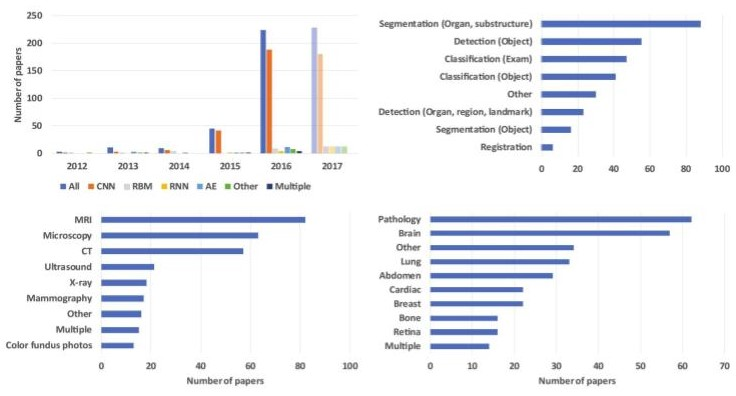
\includegraphics[width=1\textwidth]{figures/DL_CAD_statystyka.jpg}
	\caption{Statystyki dotyczące publikacji medycznych zawierających słowa kluczowe związane z głębokim uczeniem się.}
	\label{DL_CAD_stats}
\end{figure}

 Widoczny wzrost liczby publikacji nastąpił począwszy od 2015, co związane było z kilkuletnią adaptacją nowych metod w dziedzinie przetwarzania obrazów medycznych i gromadzeniem odpowiednich danych. Rok 2016 i 2017 były pod pewnym względem przełomowe gdyż pojawiało się coraz więcej prac naukowych, w których przedstawiano rezultaty dokładności klasyfikacji medycznych zbiorów danych na poziomie dorównującym ekspertom dziedzinowym.
 
 Dla przykładu, w Listopadzie 2016 ukazał się praca grupy Google Research, Mountain View, Kalifornia [https://www.ncbi.nlm.nih.gov/pubmed/27898976], gdzie zastosowano sieć GoogLeNet w wersi inception-v3 do zautomatyzowanej detekcji retinopatii cukrzycowej i cukrzycowego obrzęku plamki w obrazach dna oka. Wyniki porównano z panelem skjładającym się z 7 ekspertów, okulistów. Porównanie przedstawiono na Rys. \ref{CAD_opto}.
 \begin{figure}[h!]
 	\centering
 	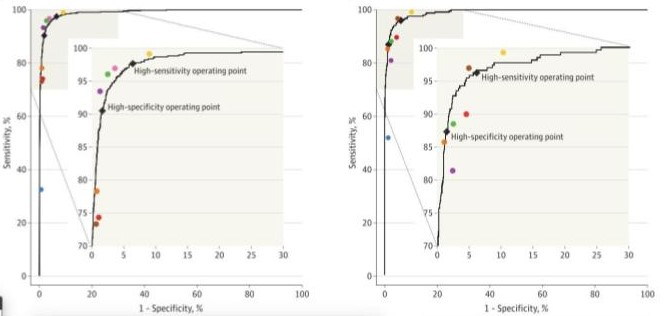
\includegraphics[width=0.7\textwidth]{figures/CAD-okulisci.jpg}
 	\caption{Porównanie automatycznej klasyfikacji retinopatii cukrzycowej i cukrzycowego obrzęku plamki z oceną panelu ekspertów}
 	\label{CAD_opto}
 \end{figure}
 
 Na wykresach dla dwóch zadań klasyfikacyjnych umieszczono krzywe reprezentujące zależność swoistości od czułości dla algorytmu automatycznego oraz 7 punktów oznaczające wynik oceny każdego z ekspertów-okulistów. Ogółem mniej niż połowa ekspertów uzyskałą lepszy wynik niż algorytm sztucznej inteligencji.
 
 Kolejna ciekawa praca pojawiła się w czasopiśmie nature w styczniu 2017 i traktowała o automatycznej detekcji raka skóry na zdjęciach [Esteva, 2017]. Autorzy wykorzystali dane składające się z 129,450 obrazów klinicznych, na których zobrazowano 2,032 różne schorzenia skóry. Ponownie do klasyfikacji wykorzystano sieć GoogleNet w wersji inception-v3. Wyniki klasyfikacji automatycznej porównano z oceną przeprowadzoną przez 21 certyfikowanych dermatologów. Przykład porównania zaprezentowano na Rys. \ref{CAD_derma}. 
 
 \begin{figure}[h!]
 	\centering
 	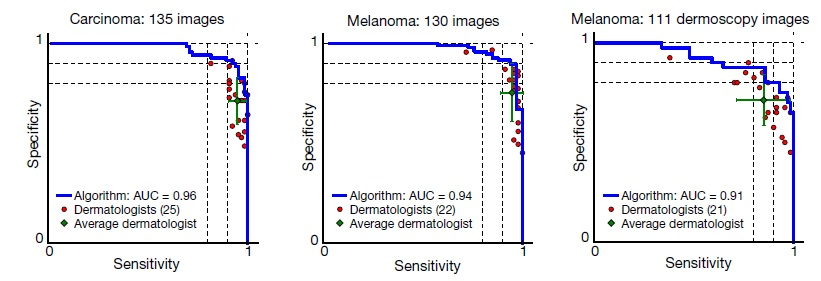
\includegraphics[width=0.9\textwidth]{figures/CAD-dermatolodzy.jpg}
 	\caption{Porównanie automatycznej klasyfikacji 3 chorób skóry z oceną ekspertów dermatologów}
 	\label{CAD_derma}
 \end{figure}

Tym razem umieszczono odwrotną zależność (tj. czułość od swoistości), czerwonymi punktami oznaczono wynik oceny ekspertów, a zielonym krzyżykiem wynik uśrednienia oceny eksperckiej. W każdym przypadku średnia ocena była gorsza od automatycznje klasyfikacji.

Obrazy medyczne nie są jedynymi danymi, które z powodzeniem są przetwarzane za pomocą metod głębokiego uczenia się. W lipcu 2017, przez grupę ze Stanford University została opublikowana praca dotycząca klasyfikacji arytmii na podstawie szeregów czasowych zapisanych na elektrokardiogramach [Rajpurkar, 2017]. Autorzy wykorzystali dane z 64,121 elektrokardiogramów, próbkowanych z częstotliwością 200 Hz, pochodzących od 29,163 pacjentów. Zaprojektowano dedykowaną, 34-warstwową sieć konwolucyjną do detekcji 12 różnych dysfunkcji pracy serca, pracy prawidłowej i szumów (łącznie 14 klas). Wyniki klasyfikacji porównano z oceną prowadzoną przez 3 kardiologów. Średnia dokładność klasyfikacji automatycznej wyniosła 80\% , natomiast manualnej 72\%.

Naturalnie, podobnych przykładów zostało opublikowanych dużo więcej. Architektura AlexNet z sukcesem była użyta do detekcji polipów w kolonospokopii [AlexNet-kolo, 2017]. Sieć ResNet sprawdziła się w badaniach w Mayo Clinic Rotschester, dotyczących radiogenomiki i rozróżnienia zmian w mózgu bez konieczności biopsji [Mayo]. Złożenia natomiast z sukcesem zostały zaaplikowany w pracach dotyczących detekcji raka płuc, gdzie modele bazowe analizowały różne skale problemu [LungChalenge]. W wielu pracach raportuje się dokładność klasyfikacji automatycznej znaczącą przewyższające możliwości dziedzinowych ekspertów np. [https://doi.org/10.1016/j.cell.2018.03.040, FNP].

 Przytoczone prace pokazują, że dla szczególnych przypadków pewien element pracy eksperta zajmującego się danymi medycznymi (np. radiologa) może być z sukcesem wspomagany przez algorytmy głębokiego uczenia się. Należy jednak podkreślić, że jest również szereg problemów wiążących się z wykorzystaniem sztucznej inteligencji w medycynie. Do najważniejszych należą:
\begin{enumerate}
	\item Gromadzenie dużych zbiorów danych z odpowiednimi etykietami.
	\item Wykorzystanie heterogenicznych danych pochodzących np. z wielu urządzeń lub modalności.
	\item Kalibracja i szacowanie niepewności wyników modelu.
	\item Unifikacja modeli wykonujących podobne zadania.
	\item Minimalizacja liczby parametrów modelu przy zachowaniu satysfakcjonującego poziomu dokładności.
\end{enumerate}

Dyskusja na temat tych problemów wciąż jest tematem wielu paneli dyskusyjnych i debat konferencyjnych np. [NVIDIA 1-2]. Najbardziej zaawansowane prace dotyczą problemu gromadzenia dużych zbiorów danych medycznych, co wymaga bliskiej współpracy ekspertów medycznych z ekspertami od uczenia maszynowego. Często konieczna jest również modyfikacja bądź tworzenie dedykowanych programów do akwizycji danych medycznych. Jako przykłady takich inicjatyw można wymienić programy Stanford Medicine [MedicalImageNet], Harward School of Medicine [10 mln images] czy Masachuset Hospital [NVIDIA 2018]. Ponadto w roku 2018 na konferencji NVIDIA GTC w San Jose (Kalifornia) Amerykańskie Stowarzyszenie Radiologii i stowarzyszenie MICCAI (od ang. \textit{Medical Image Computing and Computer Assisted Intervention}) ogłosiły porozumienie, co do wspólnej współpracy mającej na celu eliminacje barier legislacyjnych związanych ze współpracą przy pozyskiwaniu odpowiednich danych dla wykorzystania algorytmów uczenia maszynowego.

Autor tej rozprawy jest świadom ograniczeń jakie są związane z wykorzystaniem algorytmów głębokiego uczenia się. Jednocześnie, duża liczba sukcesów, które pojawiły się w ostatnich latach w aplikacjach medycznych stanowi silną motywację dla autora do przeprowadzenia własnych badań zaprezentowanych w następnym rozdziale.


    
